%%This is a very basic article template.
%%There is just one section and two subsections.
\documentclass{article}

\usepackage[utf8]{inputenc}
\usepackage[hmargin=3.0cm,vmargin=3.0cm]{geometry}
\usepackage[french]{babel}
\usepackage{graphicx}

\begin{document}

\begin{titlepage}
\vspace*{.28\textheight}
\begin{center}
%
\begin{figure}[h]
    \centering
    
\includegraphics[scale=0.12]{images/LogoSupelec}
\end{figure}
%a
\vspace*{10pt}
%\text{ }\\[7 cm]
\textbf{\LARGE{VALORISATION D'UN SUJET SCIENTIFIQUE}}\\[1 cm]
\textbf{\LARGE{\og L'Adaptation Sémantique \fg}}\\[2 cm]
Gustavo \textbf{CIOTTO PINTON}\\[1 cm]
Supélec, 2015

\end{center}
\end{titlepage}

\newpage

\section{Introduction}

L'activité de recherche est un domaine clé pour tout secteur de l'industrie, 
étant ainsi la principale source d'innovation dans une entreprise. Représentant
une branche aussi important d'une économie, une telle activité doit être
présenté pour convaincre la société de son importance. Dans ce contexte,
l'électif \og Valorisation d'un sujet scientifique \fg propose des moyens et
des techniques à attirer l'attention à notre thème. 

\vspace{12pt}

Afin d'appliquer ces concepts, rien de mieux que de savoir l'expérience d'un
professionnel qui travaille déjà dans ce secteur et, par conséquent, est déjà
habitué à participer à des conférences et à écrire des textes de nature
scientifique. Le but de ce document est donc d'explorer telles expériences.
L'interviewé, Daniel CHARLES CAFÉ, est un élève en dernière année du doctorat au
department d'informatique à Supélec.


\vspace{12pt}

Le thème choisi, la microélectronique numérique, pour ce travail a été un sujet
à mon avis très pertinent, donné son importance économique d'aujourd'hui grâce
au succès des appareils électroniques tels que les tablettes et les portables. 
La problèmatique du sujet abordé dans ce document consiste au dialogue et
à l'adaptation entre les différentes parties analogiques et numériques d'un
circuit, ce qui entraîne l'utilisation des concepts mathématiques complètement
distincts. Un des enjeux principaux du projet est alors la création d'un
simulateur capable de généraliser ces concepts à toute classe d'application,
compte tenu qu'aujourd'hui les simulateurs existants sont très complexes
et très spécifiques à une application particulière.

\section{Le sujet de la thèse de doctorat}

La simulation de systèmes mixtes, c'est-à-dire, les systèmes contenant des
parties analogique et numérique, est souvent problématique puisque les modèles
mathématiques utilisés par chacune de ces parties sont essentiellement
différents. Au côté analogique, on trouve les algorithmes classiques de
résolution d'équations différentielles qui visent à estimer la valeur de la
fonction pour chaque instant de temps.  Dans la partie numérique, d'autre part,
les événements discrets sont le principal objet d'étude d'un circuit. Prenons
l'exemple d'un circuit contenant plusieurs composants comme les diverses portes
logiques et les \textit{flips-flops}: ses états et sa sortie seront modifiés
immédiatement après du déclenchement d'un événement bien défini, généralement
représenté par un cycle d'horloge (il faut considérer quand même les
délais de propagation des signaux). Nous avons donc deux manières complètement
différentes pour effectuer les calculs, ce qui pose des problèmes considérables 
dans la construction de circuits mixtes, car, d'une part, on peut activer le
côté numérique à chaque fois qu'un calcul de la partie analogique est réalisé
ou, inversement, n'activer la partie analogique uniquement que lorsqu'un
événement discret est généré.

\vspace{12pt}

Afin de résoudre ce problème, on dispose d'une théorie appelée \og Adaptation
Sémantique \fg, qui consiste précisement à réunir les concepts appartenant à un
domaine spécifique et de les adapter à quelqu'un d'autre. Cela est réalisé
notamment en trois axes, y compris l'axe de temps, des données et de contrôle.
Sur l'axe de temps, on peut imaginer à un système responsable
pour la conversion d'un temps en secondes vers une rotation, c'est-à-dire, ce
qu'on  veut mesurer est le temps d'une rotation d'un engrenage par exemple. 
D'une part, on a la mesure en temps d'autre part, on désire qu'elle soit en
rad/s. En ce qui concerne l'adaptation de données, la conversion  est simple:
si on veut traduire une donnée analogique mesurée en volts à un niveau numérique
binaire, il est nécessaire d'introduire une direction de translation,
c'est-à-dire, on doit bien définir à partir de laquelle tension on considère le
niveau binéaire comme 0 ou 1. Bien entendu cela dépend des caractéristiques de
l'application, ou autrement dit, de la mise en œuvre de la sémantique
d'adaptation. Enfin, le dernier et l'axe le plus compliqué, celui de contrôle,
détermine la façon dont les composants seront connectés dans le circuit et la
façon dont ils se communiquent. Par exemple, nous pouvons définir , lors de la
modélisation d'un logiciel, qu'un fil répresent soit un bus de données ou soit
une queue (\textit{FIFO}). Nous pouvons également spécifier le protocole suivi
pour la transmission: \textit{Ethernet}, \textit{TCP / IP} ou quelqu'un d'autre.
En général, l'adaptation d'un axe prend en compte l'importance de chaque
composant.

\vspace{12pt}

Ces trois axes forment ainsi le centre de la théorie de l'adaptation sémantique,
qui, au début, a été développé notamment pour le domaine de l'informatique.
L'objectif de la thèse développée par mon interlocuteur est d'appliquer
justement ces concepts dans le monde de la microélectronique, spécifiquement
pour le cas de circuits mixtes.

\vspace{12pt}

Selon lui, sa première année de doctorat a été entièrement dédiéé à l'étude
des références existantes sur ce sujet, y compris les outils qui ont été déjà
mis en œuvre et les chercheurs qui y sont également intéressés. Lors de sa
recherche, Daniel a trouvé trois simulateurs qui permettaient de résoudre ce
genre de problème: la première, appelée \og MODELIX \fg~ et utilisé à Supélec,
la deuxième, \og PITOREMI \fg, a été développé à \textit{l'Université de
Berkeley} aux États-Unis et, enfin, le troisième, appelé \og SystemC \fg. Tout
d'entre eux sont basés sur des concepts relativement similaires, mais ils
traitent le problème des façons complètement différentes. Après une étude
exhaustive sur ces modèles, le doctorant a ressenti le besoin de créer, enfin,
son propre outil, en n'utilisant que les points les plus importants de chacune
de ces solutions.

\vspace{12pt}

En général, sa solution consiste à construire le schéma du circuit en haut
niveau, c'est-à-dire, sous la forme de blocs, et à ajouter à chacun de
ces composants sa respective fonction sémantique (en d'autres termes, sa
signification) - regarder figure \ref{fig:ex1}. Il faut également spécifier la
sémantique d'adaptation, qui consiste à définir la signification des fils qui relient les différents blocs du
système. Ainsi, le simulateur sait clairement ce que chaque composant
signifie et laquelle est sa fonction. Par exemple, on peut spécifier
les adaptations nécessaires que le simulateur devra tenir compte si on désire
adapter un circuit de l'analogique vers le numérique ou d'une solution
logicielle vers une matérielle.

\vspace{12pt}

\begin{figure}[h]
\centering
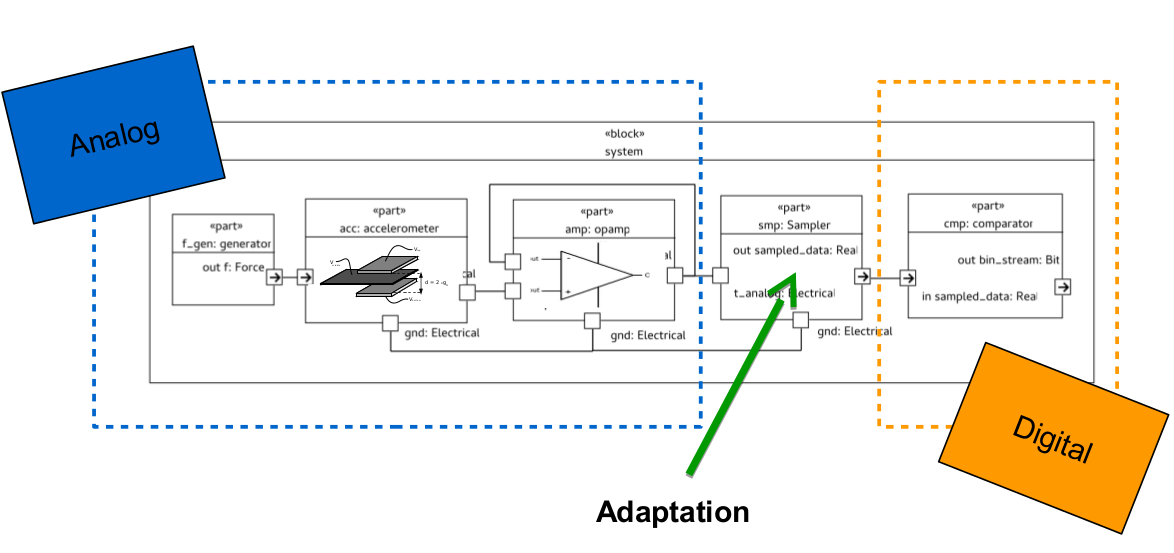
\includegraphics[scale=0.50]{images/exemple2}
\caption{Exemple modélisant l'adaptation entre systèmes continu et numérique.}
\label{fig:ex1}
\end{figure}

\vspace{12pt}

Compte tenu des caractéristiques de la solution, sa capacité de spécification se
montre comme un outil très puissant car il permet d'éviter l'utilisation de
plusieurs simulateurs différents, une fois que la solution proposée est capable
de se adapter et de simuler la communication entre les différents types de
systèmes (mécanique, électrique, analogique), et rend inutile, par conséquent,
la réalisation de calculs très lourds, impliqués dans chacun de ces systèmes.
Ainsi, la simulation de systèmes très complexes, tels que des avions ou des
voitures, dans lesquels des différents types de systèmes se communiquent en
permanence, devient plus simple et moins coûteuse. Enfin, c'est cela le secret
qui rend la valeur de cette recherche si élevée et attractive pour les
différentes entreprises d'ingénierie.

\section{La valorisation du sujet}

Dans le processus de rédaction d'un article scientifique, Daniel a remarqué
qu'une des principales difficultés est d'expliquer précisément et d'une manière
efficace le domaine de recherche d'un chercheur, qui a été profondément
analisé, pour une personne qui ne a jamais étudié ce thème. À cette fin, il a
dit qu'un document scientifique suit toujours un modèle et se compose d'une
introduction, qui sert à expliquer brièvement le problème, suivie d'une
section résumant l'état de l'art actuelle, c'est-à-dire, ce qui a été déjà
développé et comment d'autres gens ont résolu ou sont en train de le faire (y
compris les outils), le développement théorique et mathématique et, enfin, une
conclusion avec quelques perspectives futures.

\vspace{12pt}

Le doctorant m'a également expliqué que la conclusion est la partie la plus
importante d'un article et que cette section peut déterminer si l'article en
question sera lu ou pas. En d'autres termes, la conclusion doit attirer
l'attention du lecteur sur la solution de manière objective et claire. Si
la conclusion a répondu aux attentes, la section suivante à lire est
l'introduction, dans laquelle  on trouve une brève description des enjeux.
Ensuite, les autres sections sont lues en fonction des besoins du chercheur.

\vspace{12pt}

Il y a plusieurs façons de publier un article. Nous, en tant qu'ingénieurs,
avons deux objectifs principaux: d'abord, on vise les revues de l'IEEE et,
deuxièmement, de l'ACM (plutôt pour communauté du domaine informatique).
Pour les publication dans l'IEEE, la norme à être suivie consiste à séparer
le texte en deux colonnes et bien énumérer la bibliographie. Les articles
publiés dans ACM sont, par contre, écrits en une seule colonne avec la présence
de plusieurs espaces, ce qui permet l'utilisation des images par exemple.

\vspace{12pt}

Les revues possèdent également de catégories et l'importance des articles
publiés varient par rapport à elles. Les \og~\textit{journals}~\fg, une des
catégories les plus visées, sont publiés seulement une fois tous les deux ou
trois ans. Les \textit{journals} ne contiennent que les meilleures recherches
et ses articles sont plus denses, pouvant avoir plus de 20 pages chacun, puisque
le niveau de détail doit être assez élevé. Une autre alternative est de publier
des articles scientifiques de conférence, présentés de façon plus condensés et
rapide (environ 8 pages) et suivis d'une présentation tenue par d'autres
professionnels. À cet égard, il a ajouté que l'objectif de ces autres
professionnels est de vous mettre au défi de tester si votre solution est en
fait valide. Enfin, l'article passe par un dernier examen final. Si tout est OK,
l'article est publié dans les \og~ \textit{transactions} ~\fg~ et tous ceux qui
sont inscrits dans la communauté peuvent y accéder. En complément, le chercheur
peut écrire des lettres courtes, en ajoutant de petits extraits à sa recherche
(nouvelles idées, des suggestions, des résultats etc.).

\vspace{12pt}

Un autre aspect très important à considérer est aussi le type de financement
d'un doctorat. Il existe essentiellement deux options: la première, appeleé
CIFRE, se compose d'une collaboration entre l'établissement d'enseignement et la
société. Ce type d'accord est très ciblé, puisque les possibilités de développer
sa carrière dans l'entreprise sont hautes, vu que le processus de mise en œuvre
de sa solution peut prendre de nombreuses années. La deuxième forme, appelé le
CNRS, il est un financement consenti par le gouvernement et par l'école.

\section{L'interview}

À l'avis de mon interlocuteur, se conduire à la recherche dépend
de la vocation de chacun, autrement dit, un problème peut être bien résolu par
une méthode qui ne soit pas nécessairement une méthode scientifique: c'est à la
personne de choisir alors. Afin d'expliquer cette déclaration,il a cité les cas
de ~\og \textit{l'ingénierie de garage} ~\fg, typiques de la culture des
États-Unis, où la personne résout un problème particulier sans
recourir à des méthodes utilisées dans l'académie. Il remarque encore que, même
si cette personne réussit à trouver une solution à son problème, cette solution
peut ne pas être la plus efficace, car le \og chercheur \fg n'a
possiblement jamais consulté d'autres références et, ainsi, de concepts qu'elle
n'ait pensés. Ce comportement est souvent observé également dans l'industrie,
car, en cas de problème, l'ingénieur essaie naturellement de le régler en
utilisant des outils qui sont à portée de sa main. En réalisant ce type de
démarche, il risque d'oublier une étape très importante de la méthodologie
scientifique, qui est la recherche de références. Très souvent, selon Daniel,
la bonne réponse se trouve dans d'autres domaines d'activité et les communautés
(lui-même l'a fait puisqu'il est allé chercher sont sujet de doctorat dans le
domaine information, étant donné que sont vrai intêret réside dans la microélectronique).
Il conclut que le grand avantage du doctorat est l'ouverture d'esprit à
d'autres domaines: si je n'arrive pas à résoudre mes défis, alors j'ai l'option
de chercher dans un métier inconnu.

\vspace{12pt}

Daniel m'a raconté aussi une des ses expériences lors d'une conférence à
laquelle il a participé au Brésil, dont le sujet pricipal a été
précisement la difficulté de se trouver la bonne solution à un
problème particulier. Selon lui, de nombreuses personnes à travers le monde ont
les mêmes idées, mais ce qui les distingue est vraiment la capacité de mettre en
\oe uvre et de synthétiser tous les concepts dans une solution concrète.
Autrement dit, il ne s'agit seulement d'avoir les idées, mais aussi d'avoir les
connaissances techniques pour les éxecuter. En plus, il a remarqué que cette
caractéristique est fondamentelle pour le renforcement et la croissance d'une
entreprise: la capacité de s'innover en tenant en compte aussi que les
connaissances techniques sont importantes à la mesure qu'elles permettent la
mise en œuvre des idées.

\vspace{12pt} 

Toujours selon mon interlocuteur, la méthodologie industrielle est complètement
différente de celle scientifique. Dans l'industrie, lorsqu'ils se sont
confrontés à un problème, la première action est de chercher pour ceux qui vendent la
solution. Dans ce cas, il n'y a pas une vraie recherche ou étude rigoreuse du
problème. Contrairement, dans le milieu academique, les problèmes généralement
n'ont pas encore une réponse, alors la seule façon de les résoudre est par la 
méthode scientifique. C'est précisément sur cet aspect, l'art de proposer et
créer de solutions, qu'un chercheur peut évoluer professionnellement et
s'éloigner des autres,  à mesure qu'il réussit à élargir ses connaissances
à divers domaines et à publier plus de documents pertinents à la communauté.

\vspace{12pt}

Interrogé sur ses raisons de avoir réalisé son doctorat dans un pays autre que
celui de leur origine, il m'a dit que ceci était sa seule option, puisque le
domaine de la microélectronique est encore très peu développé au Brésil, son
pays d'origine. Il a également cité quelques exemples d'usines de puces à
l'étranger qui sont entièrement automatisées, tandis qu'au Brésil, les
professionnels sont obligés à les fabriquer presque manuellement.

\vspace{12pt}

Par rapport à son parcours professionnel, il m'a dit que, avant de commencer
ses activités de doctorat, il avait déjà eu une expérience au sein d'une
entreprise de microélectronique. Selon lui, cette expérience a été très
importante puisqu'elle lui a apporté des connaissances pratiques qui se sont
montrées très précieues lors de ses activités de recherche. En bref,
pour Daniel, une expérience professionnelle précédant un doctorat est
fondamentale, puisque c'est elle qui va mettre le futur chercheur en contact
avec les problèmes pratiques réels et non purement théoriques. Il a ajouté
également qu'une expérience internationale est aussi essentielle à
l'enrichissement des connaissances, puisqu'on a toujours la possibilité de
connaître d'autres façons de confronter un problème.

\vspace{12pt}

Enfin, je lui ai posé des questions à propos de l'importance d'un doctorat
lors d'une recherce d'un emploi dans les principales entreprises de la
microélectronique, comme Intel, AMD ou ARM. Il m'a répondu que, à
son avis, une thèse est très importante car elle montre le caractère innovateur
et sa capacité de poser des questions, deux caractéristiques essentielles pour
la croissance de toute entreprise.

\section{Conclusion}

L'activité de recherche assure la croissance et la réputation d'une organisation
grâce à son innovation. Ainsi, le sujet scientifique devient un aspect essentiel
à la présentation d'une nouvelle solution à une communauté particulière et doit
respecter leurs normes imposées. Par exemple, nous, en tant qu'ingénieurs,
dirigeons nos publications, dans la plupart des cas, vers les revues de l'IEEE
et de l'ACM, et par conséquent, nous devons être sûrs que notre texte répond aux
diverses impositions de telles organisations.

\vspace{12pt}

On doit également considérer l'aspect oral. Au cours de cette séquence, j'ai pu
apprendre, à travers de plusieurs exercices pratiques, les principales méthodes
qui sont actuellement utilisées pour vendre une solution. Dans ces méthodes, on
a mis en évidence l'utilisation de petits problèmes, les \og accroches \fg, et
des exemples concrets qui provoquent la réflexion des interlocuteurs. On
remarque aussi qu'il faut toujours prendre en compte les caractéristiques des
personnes avec qui on parle, pour qu'on puisse bien adapter le discours afin de
attirer leur attention plus efficacement.

\vspace{12pt} 

En ce qui concerne l'interview avec Daniel, j'ai l'impression qu'elle a
clarifié certaines questions dont je me posais par rapport à l'activité de
recherche. Je ne savais pas trop comment un professionnel décide qu'il veut un
doctorat. Avant, je pensais que ce genre d'activité a été complètement éloigné
du secteur industriel, ce qui n'est pas du tout vrai. Les deux domaines sont
complémentaires et, plus encore, dépendent les uns des autres. Par exemple, mon
interlocuteur n'a réalisé le besoin d'un doctorat qu'après avoir fait une
expérience industrielle. Sans aucun doute, actuellement un doctorat fait
désormais partie de mon projet professionnel.

\end{document}